As an example of a hybrid system described above we consider the following scenario (Figure 1): 
the ball is launched from the initial point with the initial speed $\upsilon_0$ and the angle 
to the horizon $\alpha$. When the ball reaches the ground it reflects according to the laws 
of reflection.

\begin{figure}[ht!]
\centering
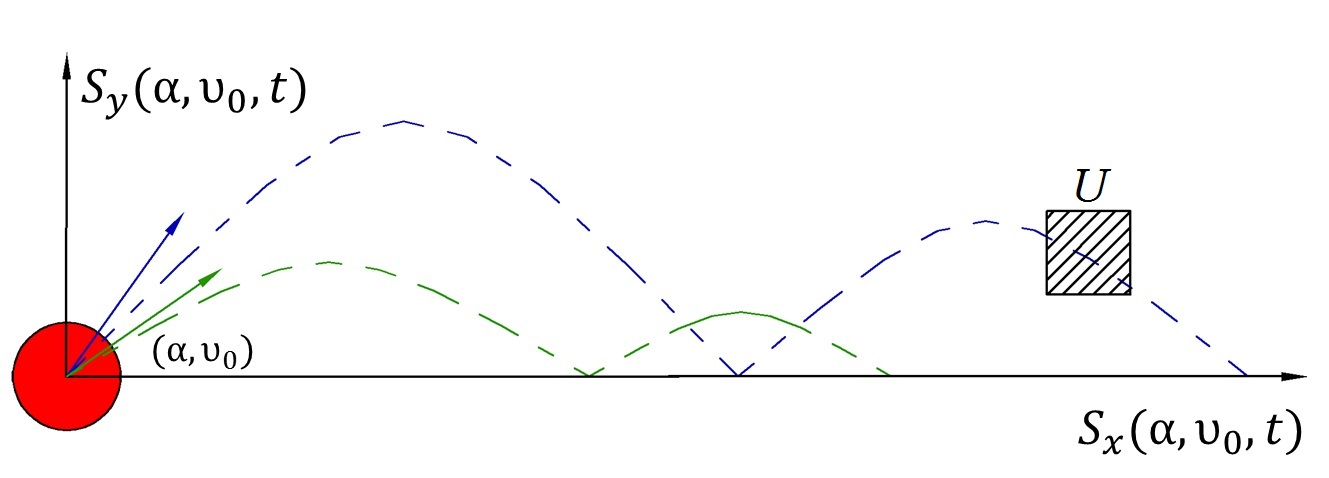
\includegraphics[width=90mm]{bouncing-ball.jpg}
\caption{Bouncing ball scenario}
\end{figure}

The ball trajectory is defined by the system of equations:
\begin{equation} \label{eq:Sx}
S_x(t) = S_{x_0} + \upsilon_0 t \cos{\alpha}
\end{equation}
\begin{equation} \label{eq:Sy}
S_y(t) = S_{y_0} + \upsilon_0 t \sin{\alpha} - \frac{g t^2}{2}
\end{equation}
where $S_x$ and $S_y$ are projections (on the axes $x$ and $y$ respectively) of the distance traveled by the ball starting at the point $(S_{x_0}; S_{y_0})$, $\upsilon_0$ is the initial speed, $\alpha$ is the angle to the horizon, $g$ is a standard gravity and $t$ is time. In this example we assume that the initial point of the ball's center is $(S_{x_0} = 0; S_{y_0} = 0)$

A hybrid system characterizing the behavior of the ball will consists of a single mode with the dynamics defined in (\ref{eq:Sx}) and (\ref{eq:Sy}) and the only jump to the same mode, during which the time $t$ is reset to $0$, the value of $S_x(t)$ before the jump is assigned to the initial value of $S_x(t)$ in the mode after the jump and the speed of the ball is reduced by the coefficient $0.9$.

In order to comply with the description of the hybrid system with random continuous initial parameters, let $\alpha$ be uniformly distributed over the interval $[0, 0.5]$ with the probability density function $f_{A}(\alpha) = 0.5$. Let $\upsilon_0 = 20$ and $t \in [0, 3]$.

Let us consider a bounded probabilistic reachability problem: \textit{is the probability that 
the system reaches in 4 steps the box $D =  \{Sx \in [90, 91], Sy \in [1, 2]\}$ greater or equal 
to $0.062$}?

The Borel set of continuous parameters is formed as:
\begin{equation*}
\begin{split}
B =\{\alpha: \exists t_{0, q_0}, t_{1, q_0}, t_{2, q_0}, t_{3, q_0} \mathord{\in} [0, T]:\\
(S_{x0} = \upsilon_0 t_{0, q_0} \cos{\alpha}) \\
\wedge (S_{y0} = \upsilon_0 t_{0, q_0} \sin{\alpha} - \frac{gt_{0, q_0}^2}{2}) \wedge 
(S_{y0} = 0) \wedge (t_{0, q_0} > 0) \\
\wedge (S_{x1} = S_{x0} + 0.9 \upsilon_0 t_{1, q_0} \cos{\alpha}) \\
\wedge (S_{y1} = 0.9 \upsilon_0 t_{1, q_0} \sin{\alpha} - \frac{gt_{1, q_0}^2}{2}) \wedge 
(S_{y1} = 0) \wedge (t_{1, q_0} > 0) \\
\wedge (S_{x2} = S_{x1} + 0.9^2 \upsilon_0 t_{2, q_0} \cos{\alpha}) \\
\wedge (S_{y2} = 0.9^2 \upsilon_0 t_{2, q_0} \sin{\alpha} - \frac{gt_{2, q_0}^2}{2})
\wedge (S_{y2} = 0) \wedge (t_{2, q_0} > 0) \\
\wedge (S_{x3} = S_{x2} + 0.9^3 \upsilon_0 t_{3, q_0} \cos{\alpha}) \\
\wedge (S_{y3} = 0.9^3 \upsilon_0 t_{3, q_0} \sin{\alpha} - \frac{gt_{3, q_0}^2}{2}) \wedge \\
(S_{x3} \in [90, 91]) \wedge (S_{y3} \in [1, 2])\}
\end{split}
\end{equation*}

Functions $S_x(\alpha, t)$ and $S_y(\alpha, t)$ are invertible with respect to $\alpha$ on 
the domain $[0, 0.5]\times[0, 3]$. Then by applying Proposition \ref{prop:ivp} the formulated 
reachability problem can be encoded as a SMT formula and solved using dReal:
\begin{multline*} 
\exists \alpha \in B = [\alpha_{min}, \alpha_{max}]:\\
(F_A'(\alpha) = f_A(\alpha)) \wedge (F_A(\alpha_{min}) = 0) \wedge (F_A(\alpha) \ge 0.062) .
\end{multline*}
The actual dReal output on the formula above was as follows:
\begin{verbatim}
SAT with the following box:
 time_0:[0.03127620501613272,
                         0.03127624003371717]
 Fa_t:[0.0625524053632542,
                         0.06255247702735234]
 Fa_0:0
 a_0:[0.4292134593911809, 0.4292134922320248]
 t_10:[1.528734841443786, 1.528734859618606]
 t_20:[1.37586135729942, 1.375861377493665]
 t_30:[1.042516533544058, 1.042516555982107]
 t_0:[1.813824229846001, 1.813824261219404]
 t_1:[1.632441880862484, 1.63244191572182]
 t_2:[1.46919748799121, 1.469197526723806]
 t_3:[0.8312598060237518, 0.8312598490599685]
 t_00:[1.698594379660991, 1.698594396018329]
 a_t:[0.4604896994248981, 0.460489732265742]
\end{verbatim}

The probability of reaching the unsafe region by the system thus falls into the interval 
$[0.0625524053632542, 0.06255247702735234]$, that is, the interval associated to the final 
value of $F_A$ (corresponding to \verb#Fa_t# in the printout above). The obtained result was 
validated using a simple Monte Carlo method in MATLAB. The time variable was discretised over 
the interval $[0, 3]$ and the system was simulated using 10,000 uniformly random samples from 
the interval $[0, 0.5]$. The number of samples hitting the unsafe region was 620, thereby 
giving a {\em probabilistic} estimate of $\frac{620}{10,000}= 0.062$. In comparison, our method 
gives an interval of size $0.72\times 10^{-7}$ which is {\em guaranteed} to contain the actual 
probability.

